\documentclass{beamer}

\usepackage[utf8]{inputenc}
\usepackage{latexsym}
\usepackage{amsmath}
\usepackage{amssymb}
\usepackage{amsthm}
\usepackage{graphicx}
\usepackage{caption}
\usepackage{hyperref}

\usetheme{Pittsburgh}
\usecolortheme{wolverine}

%% \setlength{\parindent}{2ex}

\title{Fermat's Two Squares Theorem}
\subtitle{AKA Fermat's Christmas Theorem\\A tour through two proofs}
\author{Dave Neary}
\date{April 2021}

\begin{document}

\frame{\titlepage}

\begin{frame}
	\frametitle{Outline}
	\tableofcontents
\end{frame}

\section{Fermat's statement of the Two Squares "Theorem"}

\begin{frame}
	\frametitle{Fermat's Christmas Theorem}
\begin{figure}
        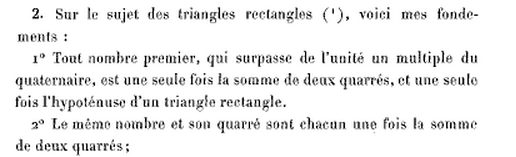
\includegraphics[width=\linewidth]{extrait_letrre_du_25_decembre_1640.png}
        \caption*{Original statement of "Fermat's Christmas Theorem"}
        \label{fig:fermat1}
\end{figure}

	Fermat wrote this statement, without proof, in a letter to Mersenne, dated December
	25th, 1640.
\end{frame}

\begin{frame}
	\frametitle{Fermat's Christmas Theorem: Statement}
	
"On the subject of right triangles, here are my findings:
	\begin{itemize}
	\item Ever prime number that is one more than a multiple of four can be written in exactly
		one way as the sum of two squares, and in one way as the hypotenuse of a right triangle
	\item The same number and its square can be written in exactly one way as the sum of two squares."
	\end{itemize}

	In modern terms: All primes of the form $4k+1$, and their squares, can be written as the sum of two
	squares of positive integers in exactly one way.
\end{frame}

\begin{frame}
	\frametitle{Which primes are sums of squares?}

	\begin{table}
\begin{tabular}{| r | c || r | c |}
	\hline 
	Primes & Sum of squares & Primes & Sum of squares \\
	\hline 
	2 & $1^2 + 1^2$ & 23 & \textcolor{red}{\textbf{\textemdash}} \\
	3 & \textcolor{red}{\textbf{\textemdash}} & 29 & $2^2 + 5^2$ \\
	5 & $1^2 + 2^2$ & 31 & \textcolor{red}{\textbf{\textemdash}} \\
	7 &  \textcolor{red}{\textbf{\textemdash}} & 37 & $1^2 + 6^2$ \\
	11 &  \textcolor{red}{\textbf{\textemdash}} & 41 & $4^2 + 5^2$ \\
	13 &  $2^2+3^2$ & 43 & \textcolor{red}{\textbf{\textemdash}} \\
	17 &  $1^2 + 4^2$ & 47 & \textcolor{red}{\textbf{\textemdash}} \\
	19 & \textcolor{red}{\textbf{\textemdash}} & 53 & $2^2 + 7^2$ \\
\hline
\end{tabular}
\caption*{The first few primes, written as sums of two squares}
\end{table}

\end{frame}

\begin{frame}
	\frametitle{Can any primes of the form $4k-1$ be a sum of squares?}

	For all integers $x,y$:
	\[ x^2, y^2 \equiv 0 \text{ or } 1 \pmod{4} \]
	\[ x^2 + y^2 \in \{0, 1, 2\} \pmod{4} \]
	Therefore:
	\[ x^2 + y^2 \not \equiv 3 \pmod{4} \]
\end{frame}


\begin{frame}
	\frametitle{Leonhard Euler, 1747}
	\begin{figure}
		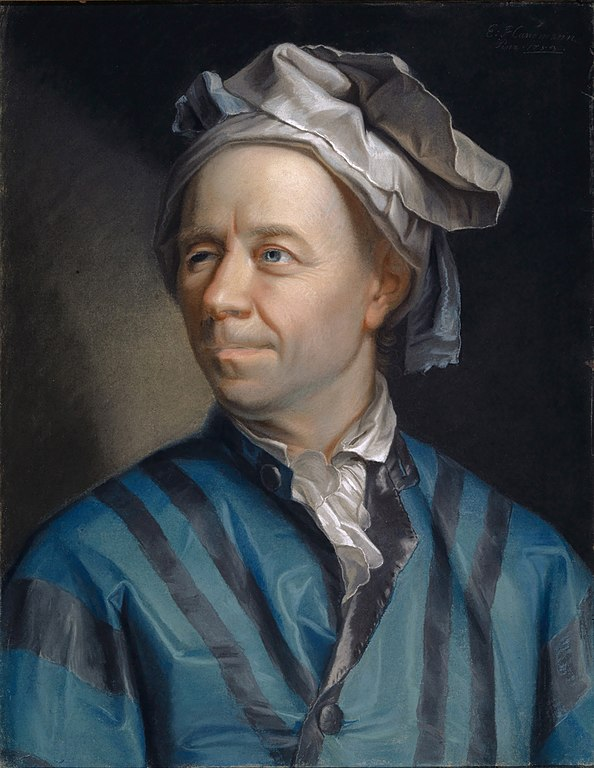
\includegraphics[width=0.3\textwidth]{594px-Leonhard_Euler.jpg}
        	\caption*{Leonard Euler}
        	\label{fig:euler1}
	\end{figure}

	The first published proof, using a method called "infinite descent" was
	published in 1747 by Leonhard Euler.
\end{frame}

%% \begin{frame}
%	\frametitle{Leonhard Euler, 1747}
%	\begin{itemize}
%		\item The sums of squares are closed under multiplication: 
%			$(a^2+b^2)(c^2+d^2) = (ac-bd)^2 + (ad-bc)^2 $
%		\item If a sum of squares is divisible by a prime of the form $p^2 + q^2$
%			then its quotient is also a sum of squares
%		\item If a sum of squares is divisible by a number which is not a sum of
%			two squares, then the quotient also has a factor which is not a
%			sum of two squares
%		\item If $a$ and $b$ are relatively prime, then every factor of $a^2+b^2$
%			is a sum of two squares
%
%	\end{itemize}
%% \end{frame}

\section{Dedekind's proof using Gaussian integers}


\begin{frame}
	\frametitle{Dedekind's proof using Gaussian Integers (1894)}
	%% \frametitle{Richard Dedekind, 1894}
	\begin{columns}
		\column{0.5 \textwidth}
		\begin{center}
			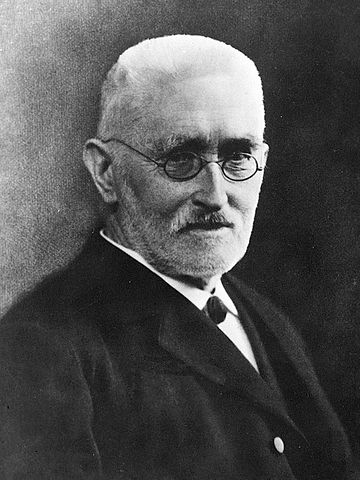
\includegraphics[width=0.8\textwidth]{Richard_Dedekind_1900s.jpg}
		\end{center}
		\column{0.5 \textwidth}
		Richard Dedekind, a German mathematician born in 1831.
		His domain of research was Number Theory, and his doctoral advisor was
		Carl Friedrich Gauss.
		
		He published two proofs of Fermat's Two Squares Theorem using the ring of
		Gaussian integers, one in 1877, and the one we will explore in 1894.

	\end{columns}
\end{frame}

\begin{frame}
	\frametitle{Gaussian Integers}
	The Gaussian integers $\mathbb{Z}[i]$ is the set 
	$\{a+ib:a, b \in \mathbb{Z}, i^2 = -1 \}$

	$\mathbb{Z}[i]$ is closed under multiplication and addition, and has additive and
	multiplicative identities.
	\begin{itemize}
		\item For $x,y \in \mathbb{Z}[i], x \times y, x + y \in \mathbb{Z}[i]$
		\item There exist elements $0, 1 \in \mathbb{Z}[i]$ such that, for all
			$x \in \mathbb{Z}[i], 0+x = x, 1 \times x = x$
	\end{itemize}
\end{frame}

\begin{frame}
	\frametitle{Factoring "primes"}

	An interesting characteristic of the Gaussian integers is that we can factor some
	expressions that do not have a factorization over the real numbers. For example:
	\[a^2 + b^2 = (a+ib)(a-ib) \]

	In this way, we can factor numbers that are prime in the natural numbers!
	\begin{align*}
		5 = 1^2 + 2^2 &= (1+2i)(1-2i) \\
		13 = 2^2 + 3^2 &= (2+3i)(2-3i)
	\end{align*}
\end{frame}

\begin{frame}
	\frametitle{Euclidean Domains}

	By defining an appropriate "norm" function $N(x)$, we can also use the Euclidean 
	division algorithm to find the GCD of elements of $\mathbb{Z}[i]$!
	\begin{itemize}
		\item Define the norm $N(a+ib) = a^2 + b^2$
		\item For all $x,y \in \mathbb{Z}[i]$, there exist $q,r \in \mathbb{Z}[i]$
			such that $x = q\times y + r$, with $N(r) < N(y)$
	\end{itemize}

	We have a way to determine prime numbers for $\mathbb{Z}[i]$
	that will be different from the primes we know in $\mathbb{N}$, and to express any
	Gaussian integer as a unique product of primes and units.
\end{frame}

\begin{frame}
	\frametitle{Euclidean division on $\mathbb{Z}[i]$}

	\only<1>{
	Let's find the GCD of $11+7i$ and $18-i$ to see how it works.
	\begin{align*}
		N(11+7i) &= 11^2 + 7^2 = 170\\
		N(18-i) &= 18^2 + 1^2 = 325 \\
		\frac{18 - i}{11+7i} &= \frac{(18-i)(11-7i)}{(11+7i)(11-7i)}\\
		&= \frac{205 - 137i}{170}
	\end{align*}
	We can round this to the nearest Gaussian integer $1-i$ to get:
	\[ 18-i = (1-i)(11+7i) + 3i \]
}
	\only<2>{
	Now we repeat the step to get:
	\[ \frac{11 + 7i}{3i} = \frac{7}{3} -\frac{11i}{3} \]
	And we round to $2-4i$:
	 \[ 11 + 7i = (2-4i)(3i) + i \]
	And since $i$ is a unit, the greatest common denominator is 1.
}

\end{frame}

\begin{frame}
	\frametitle{Fermat's Little Theorem}

	Fermat's Little Theorem states that for a prime $p$, and any number $a$ coprime with $p$ 
	(that is, $\gcd(a,p) = 1$):
	\[ a^{p-1} \equiv 1 \pmod{p} \]

	In fact, we can go further, and say that for every $a \in \mathbb{Z}/p\mathbb{Z}$, there exists
	an exponent $t$ such that $a^{e} \equiv 1 \pmod{p}$, and $e | (p-1)$. 

\end{frame}

\begin{frame}
	\frametitle{Quadratic residues}

	In modular arithmetic, a quadratic residue is a number that has a square root
	$\pmod{p}$. For example, looking at the numbers $\pmod{7}$, we see that only 0, 1, 2, 
	and 4 have square roots in $\mathbb{Z}/p\mathbb{Z}$, the numbers $\pmod{7}$.
       \begin{table}
\begin{tabular}{| l | c |}
        \hline
	$a$ & $a^2 \pmod{7}$\\
	\hline
	0 & 0 \\
	1 & 1 \\
	2 & 4 \\
	3 & 2 \\
	4 & 2 \\
	5 & 4 \\
	6 & 1 \\
	\hline
\end{tabular}
	       \caption*{Quadratic residues $\pmod{7}$}
\end{table}


\end{frame}

\begin{frame}
	\frametitle{Dedekind's proof (1)}

	From Fermat's Little Theorem, we know that $a^{p-1} \equiv 1 \pmod{p}$ for all
	$a\neq 0 \pmod{p}$. We also can show that $(-1)^{\frac{p-1}{2}} = 1$ since 
	$p = 4k-1, (-1)^{\frac{p-1}{2}} = (-1)^{2k} \equiv 1 \pmod{p}$.

	For a quadratic non-residue $a$ of $p$, the smallest power $e$ such that $a^{e} \equiv 1 \pmod{p}$
	is $e = p-1$.

	$1$ has two square roots $\pmod{p}$: itself and $-1$. Since $a^{\frac{p-1}{2}} \not \equiv 1
	\pmod{p}$, $a^{\frac{p-1}{2}} \equiv -1 \pmod{p}$.

	Therefore, for a quadratic non-residue $a$, $(a^{\frac{p-1}{4}})^2 = -1 \pmod{p}$.

\end{frame}
\begin{frame}
	\frametitle{Dedekind's proof (2)}

	If we can find a quadratic non-residue $a$, then we can set $b \equiv a^{\frac{p-1}{4}} \pmod{p}$
	and we are guaranteed that $b^2 \equiv -1 \pmod{p}$, or $p | b^2+1$.

	Factoring $b^2+1$ over $\mathbb{Z}[i]$ we get:
	\[b^2 + 1 = (b+i)(b-i) \]
	
	But since $b<p$, $N(b+i)<N(p)$, so $p$ does not divide either of these factors - which means
	that $p$ must be divisible by some other Gaussian prime factors $(n+im)(n-im) = p$.
\end{frame}

\begin{frame}
	\frametitle{Finding the squares (1)}

	We have proved that there must be some factors of $p$ in $\mathbb{Z}[i]$, but we
	have not found them. The tricky part is finding a square root of $-1$. To do this,
	we look for a quadratic non-residue of $p$ (look up "Euler's criterion", out of
	scope for this talk).

	Let's try $p=41 = 4(10+1)$ to see how it works.
	\[ 3^4 = 81 \equiv -1 \pmod{41} \]
	\[ 3^{20} = (-1)^5 \equiv -1 \pmod{41} \]
	So 3 is a non-residue of 41. Now to find a square root of -1, find $3^{10}$:
	\[ 3^{10} = 9\times(3^4)^2 \equiv 9 \pmod{41} \]
	Therefore, 41 divides $9^2 + 1 = 82$
\end{frame}

\begin{frame}
	\frametitle{Finding the squares (2)}

	We know that $41|9^2+1 = (9+i)(9-i)$. How we can find the prime factors of 41
	using the Euclidean division algorithm with either of these factors:

	\begin{align*}
		\frac{41}{9-i} &= \frac{(41)(9+i)}{9^2+1^2} \\
		 &= \frac{1}{82}(369 + 41i) \\
		41  &= 4(9-i) + (5+4i) \\
		9-i &= (1-i)(5+4i)
	\end{align*}

	We have calculated that $5+4i$, is the GCD of $41$ and $9-i$, and it is easy to
	check that $41 = 5^2 + 4^2$.

\end{frame}

\section{Zagier's "one-sentence proof"}

\begin{frame}
        \frametitle{Don Zagier, 1990}
        \begin{figure}
                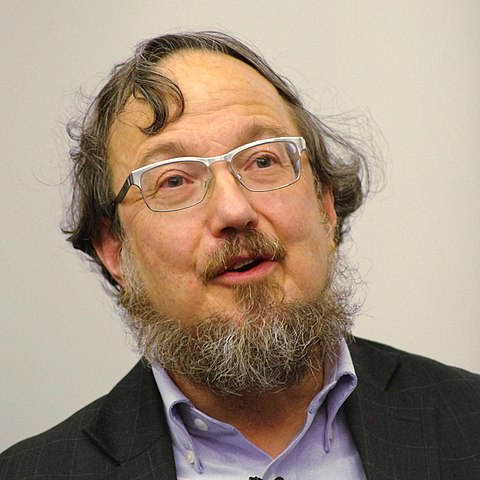
\includegraphics[width=0.4\textwidth]{480px-DonZagier-talking.jpeg}
                \caption*{Don Zagier}
                \label{fig:zagier1}
        \end{figure}

	In 1990, Don Zagier published a "one-sentence proof", based on a prior geometric proof.
\end{frame}

\begin{frame}
	\frametitle{Don Zagier proof}
	
	{\em A one-sentence proof that every prime $p\equiv 1 \pmod{4}$ is a sum of two squares.}

	The involution on the finite set $S = \{(x,y,z) \in \mathbb{N}^3:x^2+4yz = p \}$
	defined by:
	\begin{equation*}
		(x,y,z) \rightarrow
		\begin{cases}
			(x + 2z, z, y - x - z) & \text{if } x < y-z \\
			(2y - x, y, x - y + z) & \text{if } y - z < x < 2y \\
			(x - 2y, x - y + z, y) & \text{if } x > 2y
		\end{cases}
	\end{equation*}
	has exactly one fixed point, so $|S|$ is odd and the involution defined by 
	$(x,y,z) \rightarrow(x,z,y)$ also has a fixed point.

\end{frame}

\begin{frame}
	\frametitle{What!?!?!}

        \begin{center}
             
\includegraphics[width=0.8\textwidth]{side-eye-chloe.jpg}
        \end{center}

\end{frame}

\begin{frame}
	\frametitle{What is an involution?}

	An {\em involution} is a function which is its own inverse. That is:
	\[ f: A \rightarrow A : f(f(x)) = x \text{ for all } x \in A \]

	Examples:
	\begin{itemize}
		\item $ f:\mathbb{R}^+ \rightarrow \mathbb{R}^+: f(x) = \frac{1}{x} $
		\item $ f:\mathbb{R}/\{-1\} \rightarrow \mathbb{R}/\{-1\}: f(x) = \frac{1-x}{1+x} $
	\end{itemize}

\end{frame}
\begin{frame}
	\frametitle{Involutions on finite sets}

	Every involution on a finite set with an odd number of elements has at least one fixed point.

	Involutions are "swapping" functions - if you have an odd number of elements, at least one of
	the elements must not get swapped.
\end{frame}

\begin{frame}
	\frametitle{What about $S = \{x^2 + 4yz = p\}$?}

	For any prime of the form $4k+1$ we are guaranteed to find solutions of the form $x^2 + 4yz$
	for $x, y, z \in \mathbb{N}$. One obvious solution: $x=1, y=1, z=k$.

	For $p=17$:
	\begin{table}
	\begin{tabular}{|c|c|c|}
        \hline
		$x$ & $y$ & $z$ \\
        \hline
		1 & 1 & 4 \\
        	1 & 2 & 2 \\
        	1 & 4 & 1 \\
		3 & 1 & 2 \\
		3 & 2 & 1 \\
        \hline
	\end{tabular}
               \caption*{Possible values of $x,y,z$ for $p=17$}
	\end{table}

\end{frame}

\begin{frame}
	\frametitle{What about $S = \{x^2 + 4yz = p\}$?}

	\begin{columns}
	\column{0.5 \textwidth}
	For $p=17$:
	\begin{table}
	\begin{tabular}{|c|c|c|}
        \hline
		$x$ & $y$ & $z$ \\
        \hline
		1 & 1 & 4 \\
        	1 & 2 & 2 \\
        	1 & 4 & 1 \\
		3 & 1 & 2 \\
		3 & 2 & 1 \\
        \hline
	\end{tabular}
               \caption*{Possible values of $x,y,z$ for $p=17$}
	\end{table}
        \column{0.5 \textwidth}

		Notice that we get pairs of solutions when $y \neq z$ by swapping $y$
		and $z$.
	
		Also, notice that the number of solutions is odd. If we can prove it is
		{\em always} odd, then we are guaranteed at least one solution with $y=z$.

		If $y=z$, then $x^2+4yz = x^2 + (2y)^2$ is a sum of two squares, and the
		theorem is proved.
	\end{columns}

\end{frame}

\begin{frame}
	\frametitle{The complicated involution}

	\begin{equation*}
		(x,y,z) \rightarrow
		\begin{cases}
			(x + 2z, z, y - x - z) & \text{if } x < y-z \\
			(2y - x, y, x - y + z) & \text{if } y - z < x < 2y \\
			(x - 2y, x - y + z, y) & \text{if } x > 2y
		\end{cases}
	\end{equation*}

	Where did this come from? What does it represent? How do we prove that it is an involution?
\end{frame}

\begin{frame}
	\frametitle{The function is a partition}

	First, let's show that the cases are all that there are. By definition,
	$0<x,y,z \in \mathbb{N}$. If $x = y-z$ then:
	\begin{align*}
		x^2 + 4yz &= (y-z)^2 + 4yz \\
		&= y^2+2yz+z^2 \\
		&= (y+z)^2
	\end{align*}

	Similarly, if $x=2y$, then:
	\begin{align*}
		x^2 + 4yz &= (2y)^2 + 4yz \\
		&= 4y(y+z)
	\end{align*}
	In both cases, $x^2+4yz$ is not a prime.

\end{frame}

\begin{frame}
	\frametitle{Let's talk about windmills}
	\begin{center}
             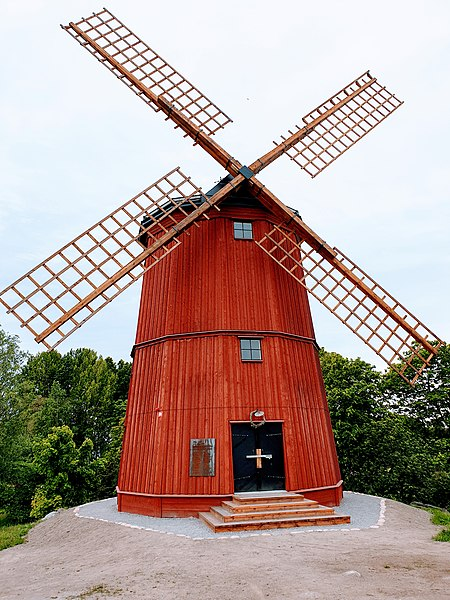
\includegraphics[width=0.5\textwidth]{windmill.jpg}
        \end{center}
\end{frame}

\begin{frame}
	\frametitle{A geometric interpretation}
	\begin{figure}
	\begin{center}
             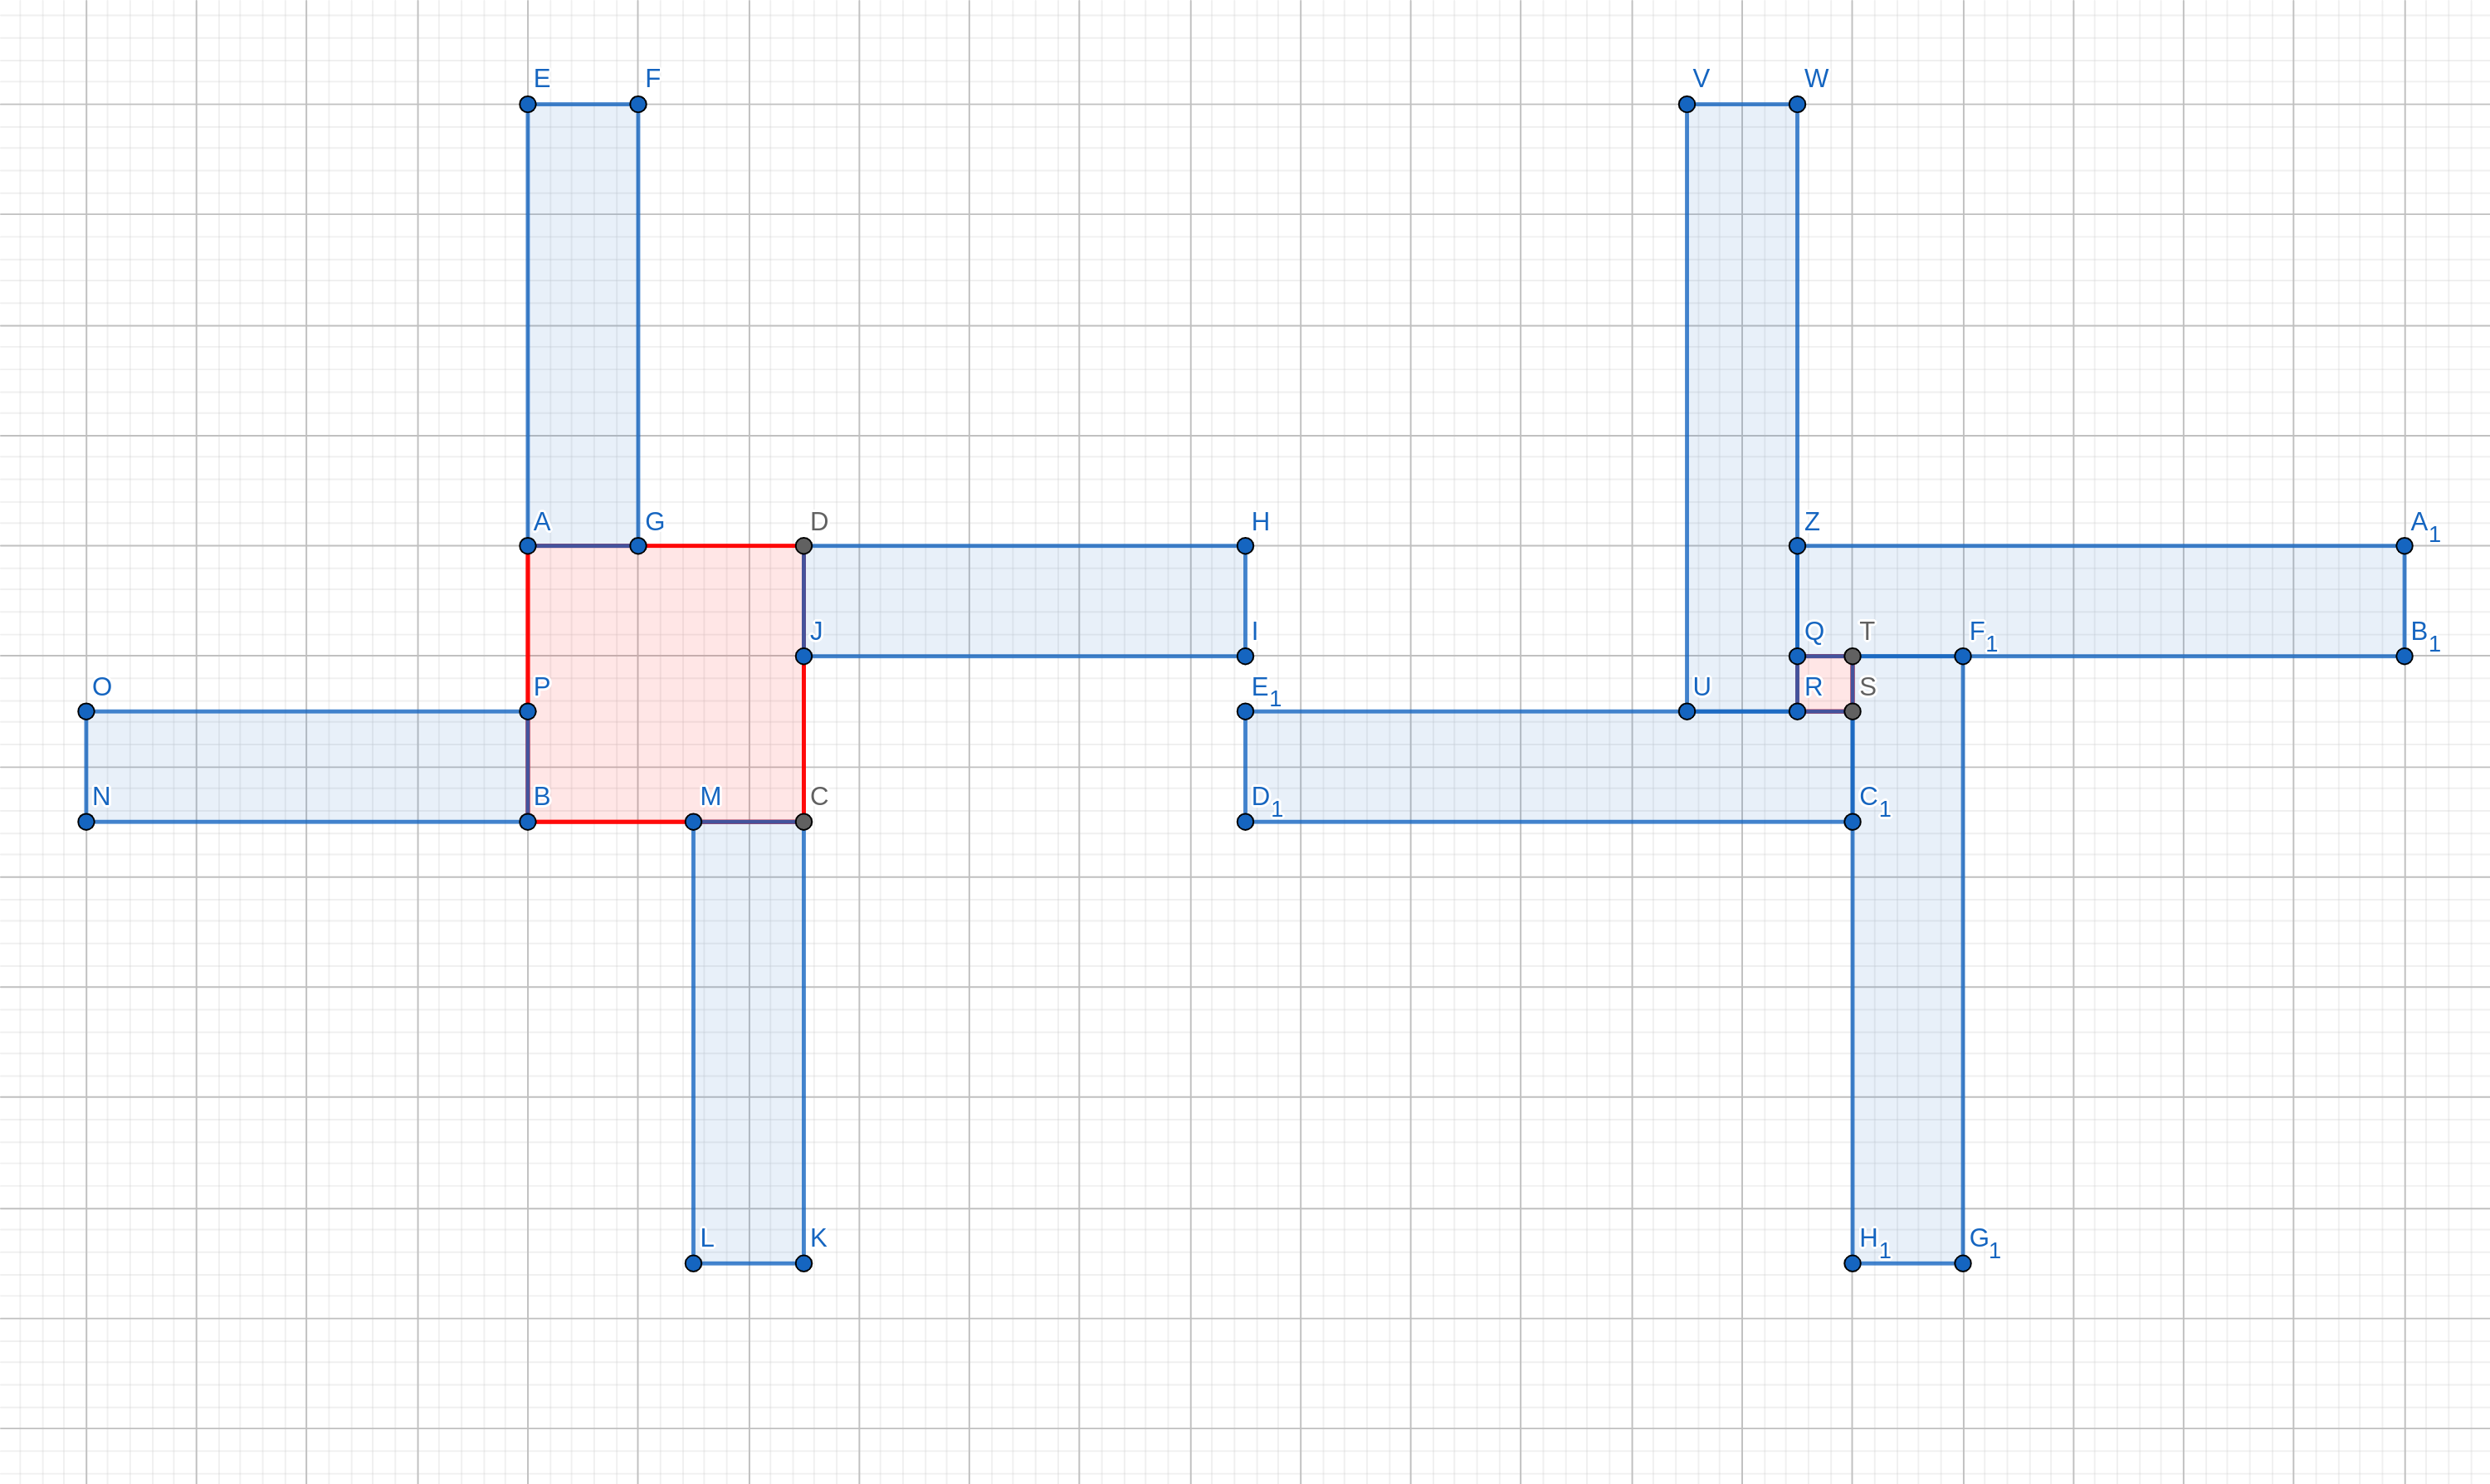
\includegraphics[width=0.8\textwidth]{windmill2.png}
        \end{center}
		\caption*{ $(5,2,8) \rightarrow (1,11,2)$}
                \label{fig:windmill2}
	\end{figure}

	We interpret $x$ as the side of a square, with $y$ the base from the top left corner and
	$z$ the height of 4 symmetrically arranged rectangles.
\end{frame}

\begin{frame}
	\frametitle{A geometric interpretation}
	The translations from one arrangement to another represent the different ways to wrap
	rectangles around a square.
	\begin{figure}
	\begin{center}
             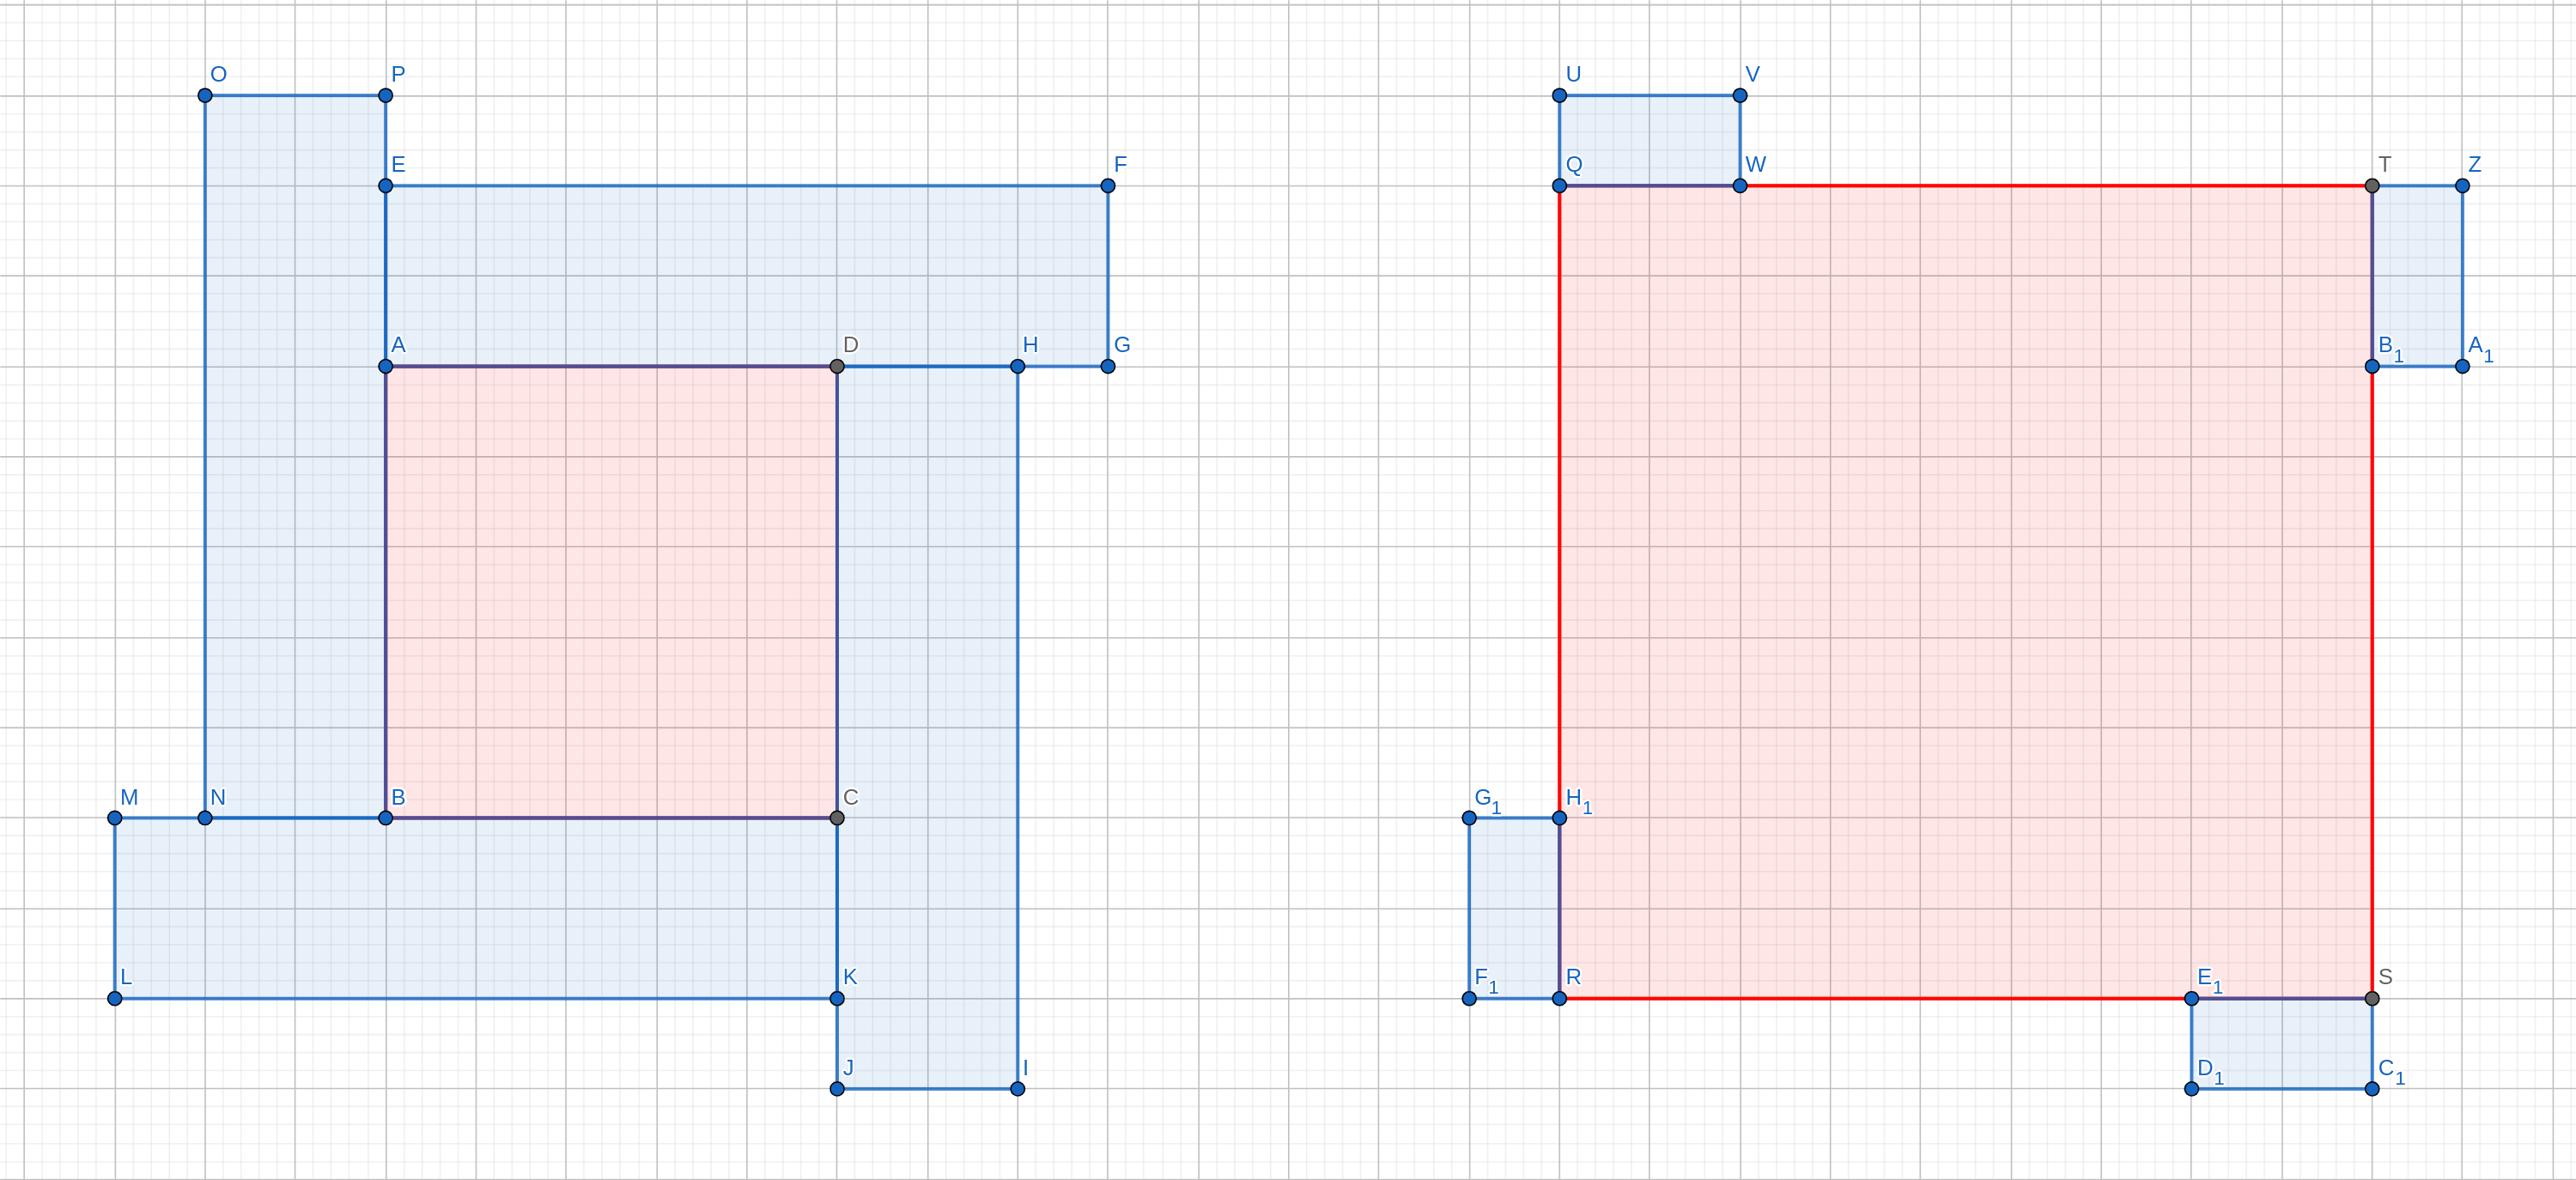
\includegraphics[width=0.8\textwidth]{windmill1.png}
        \end{center}
	\caption*{ $(5,8,2) \rightarrow (9,2,1)$}
                \label{fig:windmill1}
	\end{figure}
\end{frame}

\begin{frame}
	\frametitle{A geometric interpretation}

	Each translation represents a different type of transformation which conserves the silhouette.
	\begin{figure}
	\begin{center}
             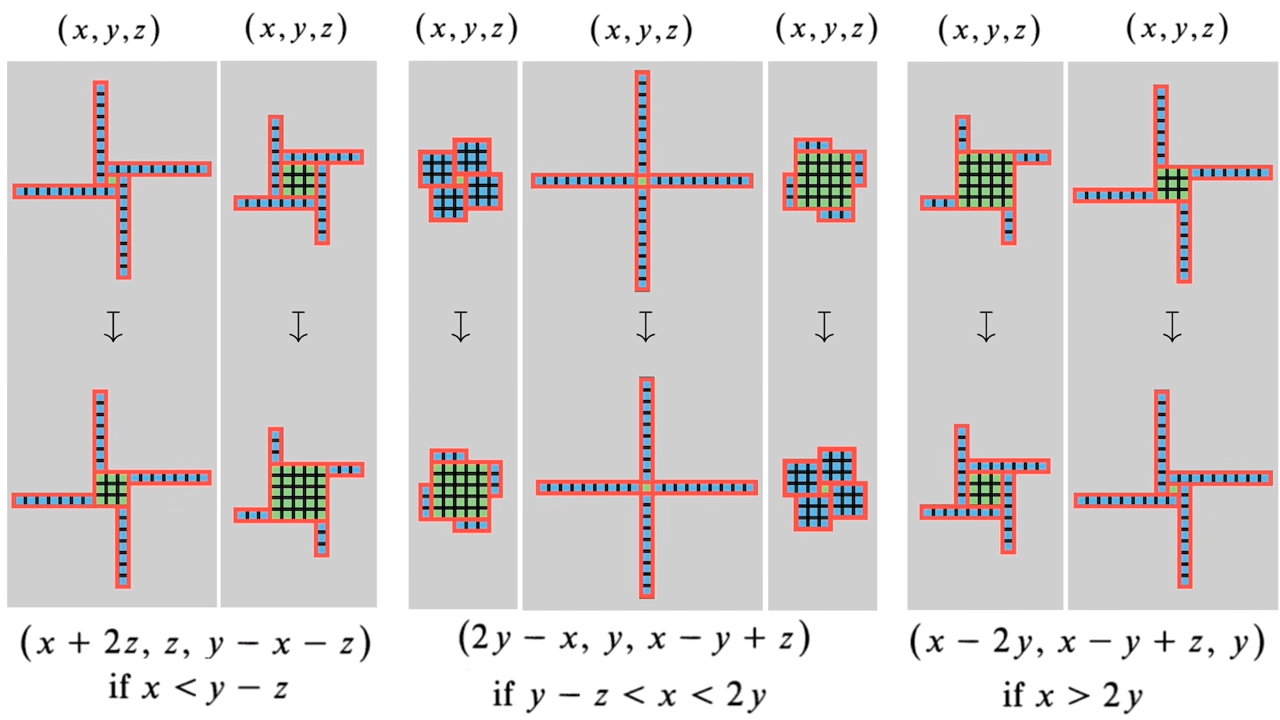
\includegraphics[width=0.8\textwidth]{windmills.png}
        \end{center}
		\caption*{All the translations (and mappings) (thank you Mathologer)}
                \label{fig:windmill_mathologer}
	\end{figure}
\end{frame}

\begin{frame}
	\frametitle{A unique fixed point}

	In all of the shapes we have seen, there are two solutions with the same silhouette. Except one.

	When $x=1, y=1, z=k$, we get a big "plus" sign. Since $y-z<x<2y$ in this case:
	\[ (1,1,k) \rightarrow (2\times 1 - 1, 1, 1 - 1 + k) = (1,1,k) \]
	is a fixed point for the mapping, and it is guaranteed to be the only one!

	Therefore, there will {\em always} be an odd number of solutions to $x^2+4yz = p$, and the
	alternative involution on the same set $(x,y,z) \rightarrow (x,z,y)$ {\em also} has a fixed
	point $y = z$.

\end{frame}

\begin{frame}
	\frametitle{Thank you! There's more! References}

	\begin{itemize}
		\item I learned about this theorem from Mathologer's awesome video about Zagier's proof:
		\href{https://www.youtube.com/watch?v=DjI1NICfjOk}{Why was this visual proof missed
		for 400 years?}

	\item You can get {\em all} the proofs of Fermat's two squares theorem (including
	a reference to a new proof from 2016!) on Wikipedia:
	\href{https://bit.ly/3gpMy7x}{Proofs of Fermat's theorem on sums of two squares}
	
	\item If you're interested in some additional materials that use Gaussian integers, you might
	enjoy 3blue1brown's video on Pythagorean triples:
	\href{https://www.youtube.com/watch?v=QJYmyhnaaek}{All possible Pythagorean triples, visualized}
	\end{itemize}
\end{frame}

\end{document}
